\begin{figure}[H]
  \centering
  \textbf{(a)}\par
  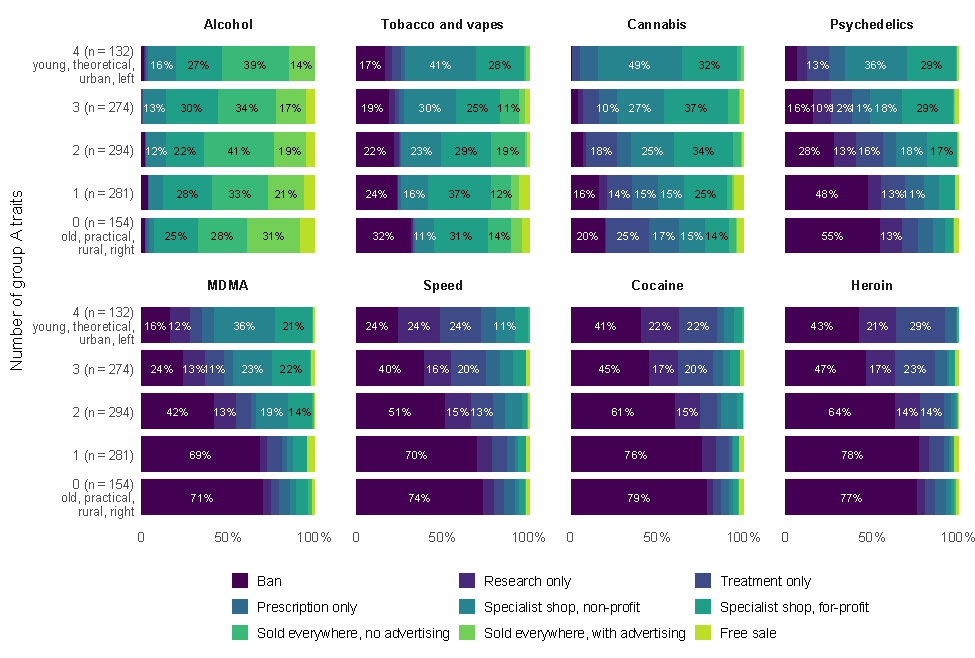
\includegraphics[width=\linewidth]{out/fig_gradient.pdf}\par\medskip
  \textbf{(b)}\par
  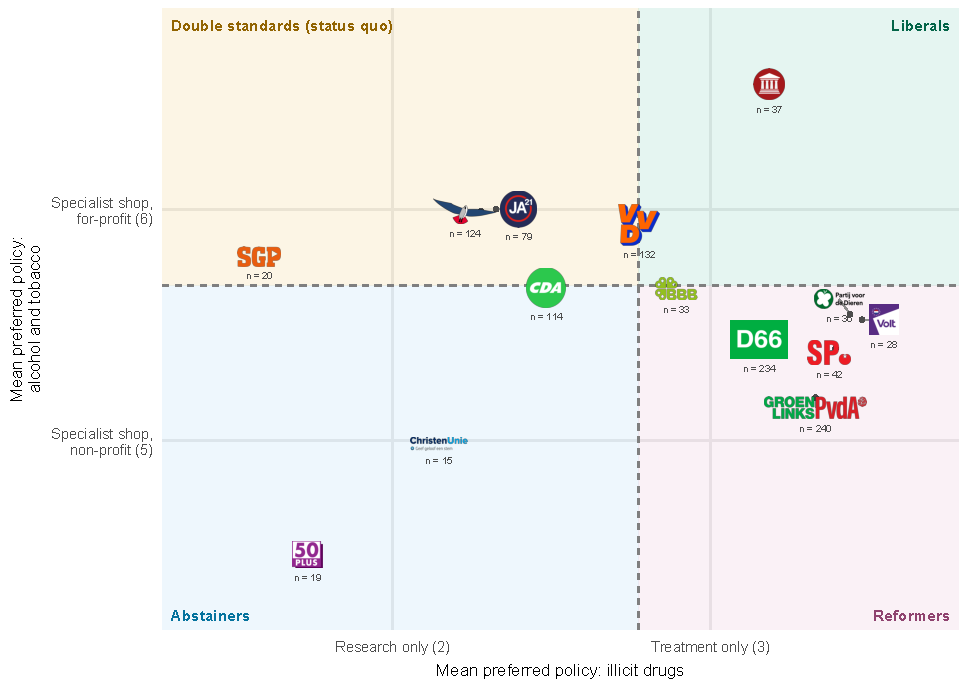
\includegraphics[width=\linewidth]{out/fig_party_map.pdf}
  \caption{\textbf{(a)} Preferred regulatory model per substance by the number of group A traits: age 18--49, theoretical education, high or very high urbanisation and a left vote. Middle education and moderate urbanisation count as not group A. Weighted shares; labels from 10\%; colours as in Figure~\ref{fig:policy_preferences}. Respondents without urbanisation or a left/right vote are left out ($n = 1135$). \textbf{(b)} Parties by support for strict regulation and for punitive measures. Horizontal: weighted share of answers in medical/research (2--4) or specialist shop (5--6), averaged per respondent over the eight substances; the dashed line is the sample mean. Vertical: mean agreement (1--7) with the four crime items, two of them reversed so that higher is more punitive ($\alpha = 0.78$; at least three items answered); the dashed line is neutral. Logo size reflects $n$ ($n = 1139$ in total); DENK ($n = 1$), other parties, blank and non-voters are left out. Vote: TK 2025. Left = GroenLinks-PvdA, D66, SP, PvdD, Volt, DENK, CU; right = PVV, VVD, CDA, JA21, FvD, BBB, 50PLUS, SGP.}
  \label{fig:gradient}
\end{figure}
